%Special definitions
\chapter{A state space model for chemical production scheduling} 
\label{chap:scheduling}
%\paragraph{Note} Most of this chapter appears in
%\citet{subramanian:maravelias:rawlings:2012}.

In Chapter \ref{chap:mpc}, we discussed design of on-line
optimization problems for the control of dynamic systems using MPC, so
that the closed-loop has desirable properties like recursive
feasibility, asymptotic convergence. In this chapter, we employ
ideas from MPC to address iterative or rolling horizon scheduling
problems.
In Section \ref{sec:scheduling:introduction}, we provide an introduction to
the problem that we wish to address. In
Section~\ref{sec:scheduling:lit_review}, we give a brief background 
on chemical production scheduling and associated rescheduling
problems. In Section~\ref{sec:scheduling:state_space}, we derive the
state space model, including four types of disturbances. In
Section~\ref{sec:scheduling:example}, we present an example
illustrating the advantages of using terminal constraints in iterative
scheduling.

\section{Introduction \footnote{This text appears in Section 1 of
\citet{subramanian:maravelias:rawlings:2012}}}
\label{sec:scheduling:introduction}

Chemical production scheduling problems arise in a wide variety of
applications, from batch production  of pharmaceuticals and fine
chemicals to continuous production of bulk chemicals and oil refining
operations. To address these problems, research within the process
systems engineering (PSE) community has primarily focused on (i) the
formulation of models for a wide variety of scheduling problems, and
(ii) the development of scheduling algorithms. In terms of model
development, the emphasis has been on the accurate representation of
problems in a range of production environments as well as the modeling
of various processing characteristics and constraints (\eg utility
constraints, changeovers, transfer operations,
etc.)\citep{mendez:cerda:grossmann:harjunkoski:fahl:2006}. An aspect
that has received limited attention is how to design algorithms, based
on these models, for iterative scheduling.

Chemical production is an inherently dynamic process. A schedule has
to be revised when new information becomes available (new orders,
modified due dates, raw material availability etc.), and/or production
disturbances occur (\eg processing delays, unit breakdowns, process
unit availability, etc.). However, while some of the issues arising when scheduling is
performed iteratively have been discussed in contributions dealing
with rescheduling, scheduling is still thought of as a {\em{static}}
open-loop problem -- the goal is to obtain an optimal schedule for the
current state of the system based on current (and possibly some
forecast) data. The development of methods (models and solution
algorithms) for the closed-loop problem has received no
attention. Another limitation of existing rescheduling methods, as we
discuss in Section~\ref{sec:scheduling:lit_review:rescheduling}, is that they are
model specific and rely on the solution of a rescheduling model that
is generated  {\em{empirically}}.

The goal of this paper is to address some of the aforementioned
limitations employing ideas from the area of control and model
predictive control (MPC) in particular. Model predictive control
offers a natural framework for the study of dynamic problems. First,
it relies on a general representation of the underlying system,
including different types of disturbances, via the state space
model. Second, it offers results with regard to the quality of the
closed-loop performance of various control strategies. For example,
with careful design of the on-line optimization problem, features such
as recursive feasibility (feasibility of the optimization problem at
each sampling instance) and asymptotic stability (convergence to a
set-point for the nominal case) can be obtained. Interestingly, it has
been shown that simple re-optimization does not necessarily lead to
good closed-loop performance, as has been assumed in the scheduling
literature.

Towards this goal, we first transform a general
mixed-integer programming (MIP) scheduling model into a state space
model \eqref{eq:mpc:cent_model}. Second, we show how common scheduling
disruptions can me modeled as disturbances in the state space model,
and finally, we discuss how some concepts from MPC like terminal
constraints can be used in scheduling. 


\section{Background}
\label{sec:scheduling:lit_review}

\subsection{Chemical production scheduling problems and models\footnote{This text appears in Section 2.1 of
\citet{subramanian:maravelias:rawlings:2012}}}


Production scheduling is one of the many planning functions in a
manufacturing supply chain. The interactions of scheduling with other
functions along with capacity considerations determine the class of
scheduling problem. The interactions with demand and production
planning determine the type of scheduling problem to be solved (cyclic
vs. short-term). The types of decisions made at the scheduling level
are determined by the decisions made at the production planning
level. Also, capacity constraints often determine the objective
function (\eg throughput maximization vs. cost minimization). Finally,
input parameters to scheduling (\eg raw material availability) are
provided by other functions \citep{maravelias:sung:2009,
  maravelias:2012, stadtler:2005}.

In general, scheduling problems can be classified in terms of a
triplet $\alpha/\beta/\gamma$, where $\alpha$ denotes the
{\emph{production}} environment; $\beta$ denotes the processing
characteristics/constraints and $\gamma$ denotes the objective
function \citep{pinedo:2008}. The main production environments are
{\emph{sequential, network}} and {\emph{hybrid}}
\citep{maravelias:2012}. Note that different types of processing can
be present in the same facility. Processing characteristics and
constraints include setups, changeovers, release/due times, storage
constraints, material transfers, etc. Common objective functions are
the minimization of makespan, the minimization of production costs,
the maximization of throughput, and the minimization of weighted lateness.

The modeling approaches to chemical production scheduling can be
classified in terms of \citep{maravelias:2012}:

\begin{enumerate}
\item the decisions made at the scheduling level;
\item the entities used to express the scheduling model; and
\item the modeling of time.
\end{enumerate}

In the most general case, scheduling involves three types of
decisions: (i) batching (number and size of batches needed to satisfy
demand); (ii) assignment of batches (or tasks) to processing units;
and (iii) sequencing and/or timing of batches (tasks) on processing
units. If the batching decisions are fixed, then scheduling problems
are expressed in terms of batches (batch-based approach). If batching
decisions are made at the scheduling level, then materials and
material amounts are typically used to formulate the scheduling model
(material-based approach). Finally, the modeling of time includes
decisions at four levels: (i) selection between precedence and
grid-based approach; (ii) if precedence-based, selection between local
and global precedences; if time-grid based, selection between common
and unit specific grids; (iii) specific assumptions regarding the
precedence relationship between two tasks and the mapping of task onto
time; and (iv) selection between discrete and continuous time
representation \citep{maravelias:2012}.

In this paper we assume batching, unit-task assignment and
sequencing/timing decisions are all made at the scheduling level
(material-based approach). We further assume that the general
scheduling problem can be expressed in terms of production
{\em{tasks, units}}(unary resources), and
{\em{materials}}. While this type of formalism has been traditionally
used to express problems in network production environment,
\citet{sundaramoorthy:maravelias:2010} showed that it can also be
employed to represent problems in all production environments. A thorough discussion of the
various scheduling problems and modeling approaches is presented in
\citet{mendez:cerda:grossmann:harjunkoski:fahl:2006}.


\subsection{Reactive scheduling\footnote{This text appears in Section 2.4 of
\citet{subramanian:maravelias:rawlings:2012}.} }
\label{sec:scheduling:lit_review:rescheduling}


Rescheduling, or reactive scheduling, after observing disturbances to
the nominal schedule has attracted some research attention in the past
few years. \citet{smith:1995} emphasizes the process view of the
scheduling problem and outlines the following criteria for {\em{reactive
scheduling}}: (i) prioritize outstanding problem; (ii) identify
modifying goals; and (iii) estimate possibilities for efficient and
non-disruptive schedule modification. In the MIP-based approaches to
reactive scheduling, a nominal schedule is used in conjunction with a
MIP model to react to disturbances. On observing a disturbance,  part
of the schedule which has already been implemented is fixed and the
remainder of the scheduling horizon is re-optimized using
modifications to the original model to reflect the disturbances. Such
strategies were proposed by
\citet{vin:jeetmanyu:ierapetritou:2000,janak:floudas:kallrath:vormbrock:2006, 
relvas:matos:barbosa:fialho:2007},  
among others. \citet{novas:henning:2010} propose a constraint
programming based approach to locally repair the nominal
solution. \citet{mendez:cerda:2003} also propose a local repair
solution to the schedule based on a MIP formulation that considers the
current ``state'' of the plant, a nominal schedule and new
information. Motivated by rolling horizon optimization in process
control, several shrinking horizon and rolling horizon approaches to
the scheduling problem have also been proposed. For instance,
\citet{van:grossmann:2003} provide an example of a complex hydrogen
pipeline, in which they divide the planning horizon into planning
periods, and for each planning period, they solve the scheduling
problem in a shrinking horizon formulation. \citet{sand:engell:2004}
solve a two stage stochastic optimization problem to find robust
schedules. They employ a moving horizon framework in which the
decisions in the current time period, the first stage decisions are
implemented, while the second stage decisions are embedded in a
scenario tree for stochastic
variables. \citet{honkomp:mockus:reklaitis:1999} use an optimizer to
perform the scheduling in conjunction with a simulator to simulate
stochastic scenarios. \citet{rodrigues:gimeno:passos:campos:1996}
propose a rolling horizon reactive scheduling method in which they
provide a predictive framework to determine future infeasibilities that
lie outside the current optimization
horizon. \citet{huercio:espuna:puigjaner:1995} present heuristics for
rescheduling based on shifting of task processing times and
reassignment of tasks to other units. \citet{li:ierapetritou:2008a}
propose a multi-parametric approach to rescheduling.
\citet{munawar:gudi:2005} propose a three level decomposition of the
problem, and motivated by process control, formulate feedback and
cascade control-like solutions to reactive
scheduling. \citet{li:ierapetritou:2008b} present a review of
different strategies used in reactive
scheduling. \citet{verderame:elia:li:floudas:2010} also present a
review of different approaches taken in different industries.



\section{State space scheduling model}
\label{sec:scheduling:state_space}

\subsection{General problem statement\footnote{ This text appears in Section 2.2 of
\citet{subramanian:maravelias:rawlings:2012}.}}


The scheduling problem we consider is stated as follows. We are given:
\begin{enumerate}
\item A set of processing tasks $i \in \mathbf{I}$; the processing time of
task $i$ is denoted by $\tilde{\tau}_i$, its fixed batchsize by
$\beta_i$ (variable batchsizes are considered in
Section~\ref{sec:scheduling:state_space:extensions}), and its production
cost by $\gamma_i$. Tasks that can be performed on many units are
modeled as different tasks, each one carried out only in one unit.
\item A set of equipment units $j \in \mathbf{J}$. The subset of tasks
  $i$ that can be carried out in unit $j$ is denoted by the set
  $\mathbf{I}_j$.
\item A set of materials $k \in \mathbf{K}$ stored in dedicated
  storage vessels of capacity $\sigma_k$. The unit inventory cost of
  $k$ is $\nu_k$. The set of tasks $i$ that produce/consume $k$ is
  denoted by $\mathbf{I}_k^+$/$\mathbf{I}_k^{-}$. Task $i$
  consumes/produces $\rho_{ik}$ units of material $k$ per unit of
  batchsize $\beta_i$. 
\item A set of shipments, $l \in \mathbf{L}$ (deliveries of feedstocks
  $k \in \mathbf{K}^F \subset \mathbf{K}$ or order for products $k \in
  \mathbf{K}^P \subset \mathbf{K}$); $\tilde{\phi}_l$ is the release
  (due) time of delivery (order) $l$; and $\zeta_l$ is the amount
  delivered ($\zeta_l > 0$) or due ($\zeta_l < 0$). $\mathbf{L}_k$ is
  the set of shipments (deliveries or orders) of material $k$. 
\end{enumerate}

Our goal is to meet the orders for the final products at the minimum
total cost. Other objective functions can also be considered.

If a task has no input or output material (\eg when two consecutive
tasks are carried out on the same unit), dummy materials can be
introduced to model the sequence of tasks. Also, if material amounts
need not be monitored (\eg sequential processes with fixed batchsize),
then we assume a nominal batchsize of 1 and unit conversion
coefficients. Note that we use the term {\emph{material}} instead of
{\emph{state}}, because the latter has a different meaning in
state space models. Raw time-related data, $\tilde{\tau}_i$ and
$\tilde{\phi}_l$ are given in regular time units (\eg hours), and are
represented by parameters with a tilde.

\subsection{Scheduling MIP model\footnote{This text appears in Section 2.3 of
\citet{subramanian:maravelias:rawlings:2012}}}

 
We consider a discrete-time model, in which the time horizon $\eta$,
is divided into $T$ periods of fixed length $\delta = \eta/T$,
defining $t+1$ time points, where period $t$ starts(ends) at time
point $t-1(t)$ \citep{shah:pantelides:sargent:1993}. We use time index
$t \in \mathbf{T}$ to denote both time point and periods. Time-related
data are scaled using $\delta$ and approximated so that the resulting
solutions are feasible. Specifically, processing times are rounded up,
$\tau_i = \lceil \tilde{\tau}_i/\delta \rceil$; and release and due
times are approximated conservatively, $\phi_l = \lceil
\tilde{\phi}_l/\delta \rceil$ if $\gamma_l >0$ and, $\phi_l = \lfloor
\tilde{\phi}_l/\delta \rfloor$ if $\gamma_l <0$. We also generate the
set of shipments for material $k$ at time $t$, $\mathbf{L}_{kt} = \set{l
  \in \mathbf{L}_k \mid \phi_l=t}$; and then calculate the total
shipment of material $k$ at time $t$:
\[ \xi_{kt} = \sum_{l \in \mathbf{L}_{kt}} \zeta_l, \qquad \forall k,t
\]
The optimizing decisions are $W_{i,t} \in \set{0,1}$ which is one if
task $i$ is assigned to start on unit $j$ at time point $t$; and
$S_{k,t} \geq 0$ , which is the inventory of material $k$ during time
period $t$. Any feasible schedule should satisfy the assignment
constraint  \eqref{eq:scheduling:assign} that expresses that at most
one task can be executed on a  unit at a time.
\begin{equation}
\label{eq:scheduling:assign}
\sum_{i \in \mathbf{I}_j}\sum_{t'=t-\tau_i+1}^{t} W_{i,t'} \leq 1,
\qquad \forall j,t
\end{equation}

If we assume that the orders are satisfied on time, the following
material balance gives the inventory variables:
\begin{equation}
\label{eq:scheduling:inventoryBalance}
S_{k,t+1} = S_{k,t} + \sum_{i\in
  \mathbf{I}_k^+}\rho_{ik}\beta_iW_{i,t-\tau_i} + \sum_{i \in
  \mathbf{I}_k^-}\rho_{ik}\beta_iW_{i,t}+ \xi_{kt} \leq \sigma_{k},
\qquad \forall k,t
\end{equation}

The objective function is 
\begin{equation}
\label{eq:scheduling:objective}
z = \min_{}{\sum_{i,t} \gamma_i W_{i,t} + \sum_{k,t}\nu_kS_{k,t}}
\end{equation}

The basic scheduling model $\mathbf{M}^{\text{SCH}}$ we consider
consists of Equations
\eqref{eq:scheduling:assign}--\eqref{eq:scheduling:objective}, with
$W_{i,t} \in \set{0,1}, \forall i,t$ and $S_{k,t} \in
[0,\sigma_k]. \forall k,t$.

If orders cannot be met on time (or we do not wish to meet them), then
we can introduce backorders variable and an additional equation for
its calculation. 

A simple problem
with one unit, two tasks and three materials, and the associated data
are shown in
Figure~\ref{fig:scheduling:ABexample}. Figure~\ref{fig:scheduling:ABgantt}
shows a solution to this problem-a Gantt chart showing the execution
of the tasks and the inventory profiles of the three materials. We use
this example throughout this chapter to illustrate the basic ideas.

\begin{figure}
  \centering
  \resizebox{0.5\columnwidth}{!}{\begin{picture}(0,0)%
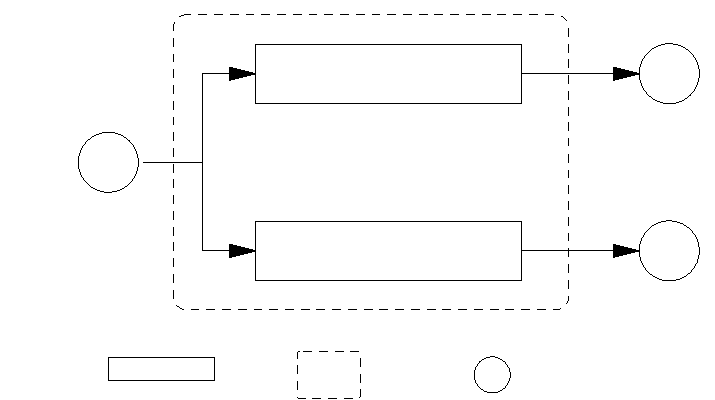
\includegraphics{scheduling/ABexample}%
\end{picture}%
\setlength{\unitlength}{4144sp}%
%
\begingroup\makeatletter\ifx\SetFigFont\undefined%
\gdef\SetFigFont#1#2#3#4#5{%
  \reset@font\fontsize{#1}{#2pt}%
  \fontfamily{#3}\fontseries{#4}\fontshape{#5}%
  \selectfont}%
\fi\endgroup%
\begin{picture}(5430,3041)(76,-3447)
\put( 91,-1726){\makebox(0,0)[lb]{\smash{{\SetFigFont{17}{20.4}{\rmdefault}{\mddefault}{\updefault}{\color[rgb]{0,.56,0}RM}%
}}}}
\put(3061,-3301){\makebox(0,0)[lb]{\smash{{\SetFigFont{17}{20.4}{\rmdefault}{\mddefault}{\updefault}{\color[rgb]{0,0,0}Unit}%
}}}}
\put(4141,-3301){\makebox(0,0)[lb]{\smash{{\SetFigFont{17}{20.4}{\rmdefault}{\mddefault}{\updefault}{\color[rgb]{0,0,0}Material}%
}}}}
\put(1801,-3301){\makebox(0,0)[lb]{\smash{{\SetFigFont{17}{20.4}{\rmdefault}{\mddefault}{\updefault}{\color[rgb]{0,0,0}Task}%
}}}}
\put(2971,-1051){\makebox(0,0)[lb]{\smash{{\SetFigFont{17}{20.4}{\rmdefault}{\mddefault}{\updefault}{\color[rgb]{0,0,0}TA}%
}}}}
\put(2971,-2401){\makebox(0,0)[lb]{\smash{{\SetFigFont{17}{20.4}{\rmdefault}{\mddefault}{\updefault}{\color[rgb]{0,0,0}TB}%
}}}}
\put(1126,-556){\makebox(0,0)[lb]{\smash{{\SetFigFont{17}{20.4}{\rmdefault}{\mddefault}{\updefault}{\color[rgb]{0,0,0}U}%
}}}}
\put(1801,-1996){\makebox(0,0)[lb]{\smash{{\SetFigFont{17}{20.4}{\rmdefault}{\mddefault}{\updefault}{\color[rgb]{0,0,0}$\tau_{TB}=2$hr, $\beta_{TB}=6$ton}%
}}}}
\put(1801,-1411){\makebox(0,0)[lb]{\smash{{\SetFigFont{17}{20.4}{\rmdefault}{\mddefault}{\updefault}{\color[rgb]{0,0,0}$\tau_{TA}=3$hr, $\beta_{TA}=4$ton }%
}}}}
\put(5491,-2401){\makebox(0,0)[lb]{\smash{{\SetFigFont{17}{20.4}{\rmdefault}{\mddefault}{\updefault}{\color[rgb]{1,0,0}$B$}%
}}}}
\put(5491,-1006){\makebox(0,0)[lb]{\smash{{\SetFigFont{17}{20.4}{\rmdefault}{\mddefault}{\updefault}{\color[rgb]{0,0,1}$A$}%
}}}}
\end{picture}%
}
  \caption{Simple scheduling problem}
  \label{fig:scheduling:ABexample}
\end{figure}

\begin{figure}[h]
  \centering
  \resizebox{0.5\columnwidth}{!}{\begin{picture}(0,0)%
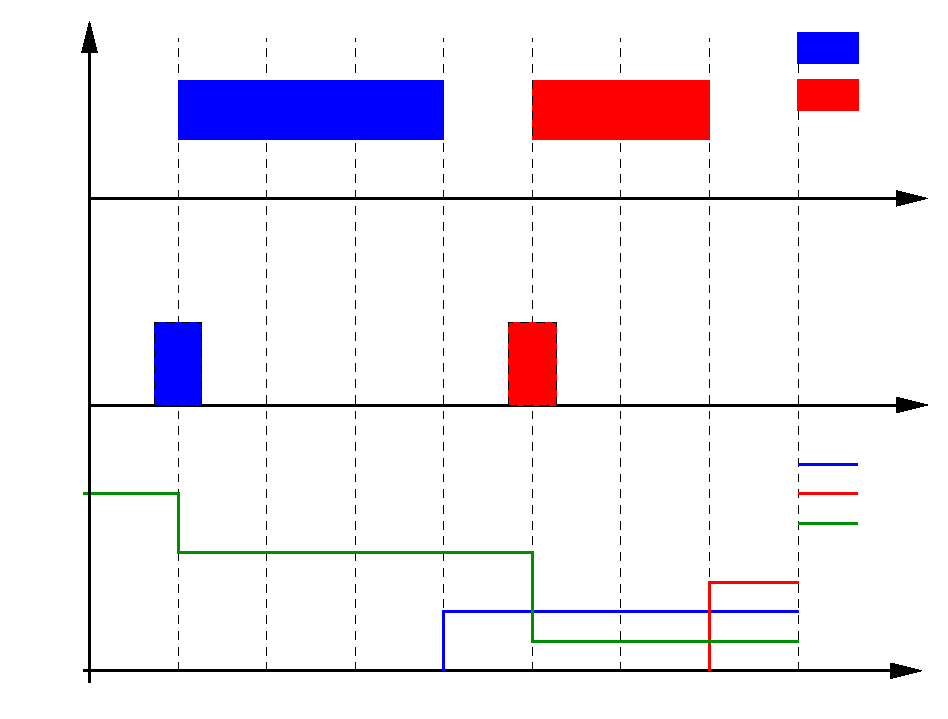
\includegraphics{scheduling/ABgantt}%
\end{picture}%
\setlength{\unitlength}{4144sp}%
%
\begingroup\makeatletter\ifx\SetFigFont\undefined%
\gdef\SetFigFont#1#2#3#4#5{%
  \reset@font\fontsize{#1}{#2pt}%
  \fontfamily{#3}\fontseries{#4}\fontshape{#5}%
  \selectfont}%
\fi\endgroup%
\begin{picture}(6967,5212)(1471,-5476)
\put(2926,-2536){\makebox(0,0)[lb]{\smash{{\SetFigFont{17}{20.4}{\rmdefault}{\mddefault}{\updefault}{\color[rgb]{0,0,0}$W_{TA,1}=1$}%
}}}}
\put(2701,-421){\makebox(0,0)[lb]{\smash{{\SetFigFont{17}{20.4}{\rmdefault}{\mddefault}{\updefault}{\color[rgb]{0,0,0}Gantt Chart}%
}}}}
\put(2701,-3571){\makebox(0,0)[lb]{\smash{{\SetFigFont{17}{20.4}{\rmdefault}{\mddefault}{\updefault}{\color[rgb]{0,0,0}Inventory profile}%
}}}}
\put(8101,-556){\makebox(0,0)[lb]{\smash{{\SetFigFont{17}{20.4}{\rmdefault}{\mddefault}{\updefault}{\color[rgb]{0,0,0}TA}%
}}}}
\put(8101,-916){\makebox(0,0)[lb]{\smash{{\SetFigFont{17}{20.4}{\rmdefault}{\mddefault}{\updefault}{\color[rgb]{0,0,0}TB}%
}}}}
\put(7966,-3706){\makebox(0,0)[lb]{\smash{{\SetFigFont{17}{20.4}{\rmdefault}{\mddefault}{\updefault}{\color[rgb]{0,0,0}$S_{A,t}$}%
}}}}
\put(7966,-3931){\makebox(0,0)[lb]{\smash{{\SetFigFont{17}{20.4}{\rmdefault}{\mddefault}{\updefault}{\color[rgb]{0,0,0}$S_{B,t}$}%
}}}}
\put(7966,-4156){\makebox(0,0)[lb]{\smash{{\SetFigFont{17}{20.4}{\rmdefault}{\mddefault}{\updefault}{\color[rgb]{0,0,0}$S_{RM,t}$}%
}}}}
\put(1486,-2356){\makebox(0,0)[lb]{\smash{{\SetFigFont{17}{20.4}{\rmdefault}{\mddefault}{\updefault}{\color[rgb]{0,0,0}$W_{i,t}$}%
}}}}
\put(7831,-5461){\makebox(0,0)[lb]{\smash{{\SetFigFont{17}{20.4}{\rmdefault}{\mddefault}{\updefault}{\color[rgb]{0,0,0}Time}%
}}}}
\put(3376,-5416){\makebox(0,0)[lb]{\smash{{\SetFigFont{17}{20.4}{\rmdefault}{\mddefault}{\updefault}{\color[rgb]{0,0,0}2}%
}}}}
\put(4726,-5416){\makebox(0,0)[lb]{\smash{{\SetFigFont{17}{20.4}{\rmdefault}{\mddefault}{\updefault}{\color[rgb]{0,0,0}4}%
}}}}
\put(6076,-5416){\makebox(0,0)[lb]{\smash{{\SetFigFont{17}{20.4}{\rmdefault}{\mddefault}{\updefault}{\color[rgb]{0,0,0}6}%
}}}}
\put(7426,-5416){\makebox(0,0)[lb]{\smash{{\SetFigFont{17}{20.4}{\rmdefault}{\mddefault}{\updefault}{\color[rgb]{0,0,0}8}%
}}}}
\put(5626,-2536){\makebox(0,0)[lb]{\smash{{\SetFigFont{17}{20.4}{\rmdefault}{\mddefault}{\updefault}{\color[rgb]{0,0,0}$W_{TB,5}=1$}%
}}}}
\end{picture}%
}
  \caption{Scheduling solution}
  \label{fig:scheduling:ABgantt}
\end{figure}


\subsection{Inputs and states\footnote{This section corresponds to the model developed in Section 3.1 of
  \citet{subramanian:maravelias:rawlings:2012}.}}
 
%\paragraph{Note:} This text appears in Section 3.1 of
%\citet{subramanian:maravelias:rawlings:2012}. 

Since assignment variables $W_{i,t}$ are the main scheduling
decisions; they are the inputs in the state space realization of $\mathbf{M}^{\text{SCH}}$. Inventory
levels $S_{k,t}$ in $\mathbf{M}^{\text{SCH}}$ are determined by
$W_{i,t}$ and the inventory balance dynamics, and hence are states. However, the
variables $S_{k,t}$ do not completely describe the state of the
system. Consider the solution shown in Figure
\ref{fig:scheduling:ABgantt}. The variables $W_{\text{TA},2}$ and
$W_{\text{TA},3}$  are both zero, but at $t=2$, the task TA has run for
one hour while at $t=3$, the task TA has run for two hours. Therefore,
to completely describe the state of the system, the history of the
system should also be included in the system state. This is achieved
through {\em{lifting}}.  We define the new state variables
$\bar{W}_{i,t}^{n}$ to carry past decisions to $t$. The state variable
$\bar{W}_{i,t}^{n} = 1$ indicates that a batch of task $i$ started at
time $t-n$. The lifted equations are given by:
\begin{align}
\label{eq:scheduling:liftedW}
\bar{W}_{i,t+1}^{1} &= W_{i,t} \nonumber \\
\bar{W}_{i,t+1}^{n} &= \bar{W}_{i,t}^{n-1} \quad \forall n \in
\set{2,3,\ldots,\tau_i}  
\end{align}

Using the lifted states, the inventory balance equation
\eqref{eq:scheduling:inventoryBalance} can be written as:

\begin{equation}
\label{eq:scheduling:x}
S_{k,t+1} = S_{k,t} + \sum_{i\in
  \mathbf{I}_k^+}\rho_{ik}\beta_i\bar{W}_{i,t}^{\tau_i} + \sum_{i\in
  \mathbf{I}_k^-}\rho_{ik}\beta_iW_{i,t}+ \xi_{k,t} \qquad \forall k,t
\end{equation}

Similarly, the assignment constraint \eqref{eq:scheduling:assign} can
be written as
\begin{equation}
\label{eq:scheduling:constraint}
\sum_{i \in \mathbf{I}_j} W_{i,t} + \sum_{i \in \mathbf{I}_j}
\sum_{n=1}^{\tau_i-1}\bar{W}_{i,t}^{n} \leq 
1 \qquad \forall j,t
\end{equation}

Defining the state $x(t) = \begin{bmatrix}S_{k,t}, k \in \mathbf{K}, &
\bar{W}_{i,t}^{n}, i \in \mathbf{I}, n \in
\set{1,2,\ldots,\tau_i} \end{bmatrix}$, the input $u(t)
= \begin{bmatrix} W_{i,t}, i \in \mathbf{I}\end{bmatrix}$ and the 
disturbance $d(t) = \begin{bmatrix} \xi_{k,t}, k \in
  \mathbf{K}\end{bmatrix}$, we can write the 
  scheduling model in the familiar state space form $x(k+1) = 
Ax(k)+Bu(k)+B_dd(k)$. Equations \eqref{eq:scheduling:liftedW} and 
\eqref{eq:scheduling:x} express the dynamic evolution of the system, 
and Equation \eqref{eq:scheduling:constraint} is a joint state-input
constraint. The objective function can be easily written as the sum of
economic stage costs $\ell_E(x,u) = q'x+r'u$.

The dynamic evolution, constraints and stage costs for the simple
scheduling model introduced in Figure \ref{fig:scheduling:ABexample}
are given in Equations
\eqref{eq:scheduling:ABss}--\eqref{eq:scheduling:ABstage_cost}.


\begin{equation}
\label{eq:scheduling:ABss}
\begin{bmatrix}S_{\text{RM}}\\S_A\\S_B\\\bar{W}_{\text{TA}}^1\\ 
\bar{W}_{\text{TA}}^2\\\bar{W}_{\text{TA}}^3\\\bar{W}_{\text{TB}}^1
\\\bar{W}_{\text{TB}}^2\end{bmatrix}_{t+1}
= \underbrace{\begin{bmatrix}
 1& & & & & & & \\
 &1 & & & &\beta_{\text{TA}} & & \\ 
 & &1 & & & & &\beta_{\text{TB}} \\
 & & & & & & & \\
 & & & &1 & & & \\
 & & & & &1 & & \\
 & & & & & & & \\
 & & & & & &1
 & \end{bmatrix}}_{A}\underbrace{\begin{bmatrix}S_{\text{RM}}\\
S_A\\S_B\\\bar{W}_{\text{TA}}^1\\\bar{W}_{\text{TA}}^2\\
\bar{W}_{\text{TA}}^3\\\bar{W}_{\text{TB}}^1\\
\bar{W}_{\text{TB}}^2\end{bmatrix}_{t}}_{x(t)}+
\underbrace{
\begin{bmatrix}
-\beta_{\text{TA}} & -\beta_{\text{TB}}\\
 & \\
 & \\
1 & \\
 & \\
 & \\
 &1 \\
 & \end{bmatrix}
}_{B}\underbrace{\begin{bmatrix}W_{\text{TA}}
    \\W_{\text{TB}}\end{bmatrix}_{t}}_{u(t)} +
\underbrace{
\begin{bmatrix}
 & \\
1 & \\
 &1 \\
 & \\
 & \\
 & \\
 &\\
 & \end{bmatrix}
}_{B_d}\underbrace{\begin{bmatrix}\xi_{A}\\\xi_{B}\end{bmatrix}_{t}}_{d(t)} 
\end{equation}

\begin{equation}
\label{eq:scheduling:ABconst}
\begin{bmatrix} 0 \\ 0 \\ 0\\ 0 \end{bmatrix} \leq
\underbrace{
\begin{bmatrix}
1& & & & & & & \\
 &1& & & & & & \\
 & &1& & & & & \\
 & & &1&1& &1& \end{bmatrix}   
}_{E_x}
\begin{bmatrix}S_{\text{RM}}\\S_A\\S_B\\
\bar{W}_{\text{TA}}^1\\\bar{W}_{\text{TA}}^2\\
\bar{W}_{\text{TA}}^3\\\bar{W}_{\text{TB}}^1\\
\bar{W}_{\text{TB}}^2\end{bmatrix}_{t}+
\underbrace{
\begin{bmatrix}
 & \\
 & \\
 & \\
1& 1 \end{bmatrix}
}_{E_u}\begin{bmatrix}W_{\text{TA}}
    \\W_{\text{TB}}\end{bmatrix}_{t} \leq 
\begin{bmatrix}\sigma_{\text{RM}}\\\sigma_{A}\\
\sigma_{B}\\1\end{bmatrix}
\end{equation}
\begin{equation}
\label{eq:scheduling:ABstage_cost}
\ell_E(x,u)
= \underbrace{\begin{bmatrix}\nu_{\text{RM}} & \nu_A & \nu_B & & &
  & \end{bmatrix}}_{q'}\begin{bmatrix}S_{\text{RM}}\\
S_A\\S_B\\\bar{W}_{\text{TA}}^1\\  
\bar{W}_{\text{TA}}^2\\\bar{W}_{\text{TA}}^3\\
\bar{W}_{\text{TB}}^1\\\bar{W}_{\text{TB}}^2\end{bmatrix}_{t}+   
\underbrace{\begin{bmatrix}\gamma_{\text{TA}} 
  & \gamma_{\text{TB}} \end{bmatrix}}_{r'}\begin{bmatrix}W_{\text{TA}}
    \\W_{\text{TB}}\end{bmatrix}_{t}
\end{equation}

\subsection{Disturbances\footnote{This section corresponds to the model developed in Section 3.1 of
  \citet{subramanian:maravelias:rawlings:2012}.} }

Events that can lead to rescheduling are modeled as disturbances. We
have already discussed shipments as a disturbance in the previous
section. In this section, we model three disturbances, namely, task yields, task
delays and unit breakdowns. 

\subsubsection{Shipments}
We assume that backorders are not allowed. Therefore, the shipping
schedule is fixed by customer orders. Hence, shipments are treated as
disturbances. We denote the nominal customer demands as
${\xi}_{k,t}^{\text{nom}}$. Shipment disturbances are deviations
$\hat{\xi}_{k,t}$ from the nominal value. That is,
\[ \xi_{k,t} = \xi_{k,t}^{\text{nom}} + \hat{\xi}_{k,t} \] 


\subsubsection{Task yields}
Consumption and production disturbances are used to model changes in
yields and losses during loading and
unloading. We define  yield disturbance variables $\beta_{i,k,t}^P$
and $\beta_{i,k,t}^C$ to denote deviation from the nominal
production/consumption of material $k$ by a batch of task $i$
finishing/starting at time $t$. For example, $\beta_{i,k,t}^P < 0$
indicates lower yield than the nominal batch size. The material
balance equations \eqref{eq:scheduling:x} is now modified as :

\begin{equation}
\label{eq:scheduling:yield_loss}
S_{k,t+1} = S_{k,t} + \sum_{i\in
  \mathbf{I}_k^+}\rho_{ik}\beta_i\bar{W}_{i,t}^{\tau_i} + \sum_{i\in
  \mathbf{I}_k^-}\rho_{ik}\beta_iW_{i,t}+ \left(\xi_{k,t} + \sum_{i\in
  \mathbf{I}_k^+}\rho_{ik}\beta_{i,k,t}^{P} +\sum_{i\in
  \mathbf{I}_k^-}\rho_{ik}\beta_{i,k,t}^{C}\right)    \qquad \forall k,t
\end{equation}

\subsubsection{Task delays}
We introduce
disturbance variable $\hat{Y}_{i,t}^{n}$ to model delays during the
execution of a task. The variable $\hat{Y}_{i,t}^{n} = 1$ when an 1-period delay
($\delta$ h) of task $i$ occurring $n$ periods after task $i$
started has been observed. The state equations ~\eqref{eq:scheduling:liftedW} are corrected as:

\begin{align}
\label{eq:scheduling:task_delay_W}
\bar{W}_{i,t+1}^{1} &= W_{i,t} - \hat{Y}_{i,t} \nonumber \\
\bar{W}_{i,t+1}^{n} &= \bar{W}_{i,t}^{n-1} + \hat{Y}_{i,t}^{n} -
\hat{Y}_{i,t}^{n-1},\qquad \forall i,t,n \in \set{2,3,\ldots,\tau_i}
\end{align}

Equation \eqref{eq:scheduling:task_delay_W} essentially says that the
values of states $\bar{W}_{i,t+1}^{n}$ should be the same as
$\bar{W}_{i,t}^{n}$ if there is a 1-period delay at $t$.  The state
equations \eqref{eq:scheduling:x} is corrected as:

\begin{equation}
\label{eq:scheduling:task_delay_S}
S_{k,t+1} = S_{k,t} + \sum_{i\in
  \mathbf{I}_k^+}\rho_{ik}\beta_i\bar{W}_{i,t}^{\tau_i} + \sum_{i\in
  \mathbf{I}_k^-}\rho_{ik}\beta_iW_{i,t}+ \xi_{k,t} - \sum_{i\in
  \mathbf{I}_k^+}\rho_{ik}\beta_i\hat{Y}_{i,t}^{\tau_i}    \qquad \forall k,t
\end{equation}

For example, consider the situation in which the task $\text{TA}$ was
started at $t=1$. Hence $W_{\text{TA},1} = 1$. The state equation
\eqref{eq:scheduling:liftedW}, then implies that
$\bar{W}_{\text{TA},3}^{2} = 1$, as at $t=3$, the task $\text{TA}$ has
been running for $2$ hours. If a 1-period delay is observed at time
$t=3$, then the variable $\hat{Y}_{\text{TA},3}^{2} = 1$. This means that
instead of finishing at $t=4$, the task gets completed only at
$t=5$. Hence, for modeling purpose, the task started only at time
$t=2$. In rescheduling literature, a new model is written with this
information, i.e., $W_{\text{TA},2}=1, W_{\text{TA},1}=0$. In our
proposed method, such delays are handled organically by modifying the
lifted states. Equation \eqref{eq:scheduling:task_delay_W} tells us
that
\[ \bar{W}_{\text{TA},4}^{3} = \bar{W}_{\text{TA},3}^{2} +
\hat{Y}_{\text{TA},3}^{3} -\hat{Y}_{\text{TA},3}^{2} = 1+0 -1 = 0 \]
and 
\[ \bar{W}_{\text{TA},4}^{2} = \bar{W}_{\text{TA},3}^{1} +
\hat{Y}_{\text{TA},3}^{2} -\hat{Y}_{\text{TA},3}^{1} = 0+1-0 = 1\]
Hence, we can verify that the disturbance variable $\hat{Y}_{i,t}^{n}$
successfully models an 1-period delay. 

\subsubsection{Unit breakdowns}
In contrast to a  task delay, a unit breakdown leads to the termination of the
task being executed on the unit at the time of the breakdown. In such
an event, all production in that unit is also lost.  To model a breakdown of unit $j$, we introduce
disturbance variable $\hat{Z}_{i,t}^{n}$. The variable
$\hat{Z}_{i,t}^{n} = 1$ when a breakdown (of duration 1 period)
occurring $n$ hours after task $i \in \mathbf{I}_j$ started is observed.
Unlike the previous section, we force all the lifted variables
affected by the shutdown to be zero as:
\begin{align}
\label{eq:scheduling:breakdown_W}
\bar{W}_{i,t+1}^{1} &= W_{i,t} - \hat{Z}_{i,t} \nonumber\\
\bar{W}_{i,t+1}^{n} &= \bar{W}_{i,t}^{n-1} - \hat{Z}_{i,t}^{n-1} \qquad
\forall i, n \in \set{2,3,\ldots,\tau_i}
\end{align}

The  state equations \eqref{eq:scheduling:x} is corrected as
\begin{equation}
\label{eq:scheduling:breakdown_S}
S_{k,t+1} = S_{k,t} + \sum_{i \in
  \mathbf{I}_k^+}\rho_{ik}\beta_i\bar{W}_{i,t}^{\tau_i} + \sum_{i\in
  \mathbf{I}_k^-}\rho_{ik}\beta_iW_{i,t}+ \xi_{k,t} - \sum_{i\in
  \mathbf{I}_k^+}\rho_{ik}\beta_i\hat{Z}_{i,t}^{\tau_i}    \qquad \forall k,t
\end{equation}

Finally, to ensure that no tasks are assigned to unit $j$ if it is out
of order, the constraint \eqref{eq:scheduling:constraint} is modified as:

\begin{equation}
\label{eq:scheduling:breakdown_constraint}
\sum_{i \in \mathbf{I}_j} W_{i,t} + \sum_{i \in \mathbf{I}_j}
\sum_{n=1}^{\tau_i-1}\bar{W}_{i,t}^{n} +\sum_{i \in \mathbf{I}_j}
\sum_{n=1}^{\tau_i-1}\hat{Z}_{i,t}^{n}  + \hat{Z}_{i,t} \leq 
1 \qquad \forall j,t
\end{equation}

A breakdown lasting multiple periods, from $t$ to $t+\phi$ can be
modeled as consecutive 1 period breakdowns. Since the subsequent
breakdowns occur while no task is executed, we introduce an idle task
$\text{IT}(j) \forall j$ with $ \tau_{\text{IT}(j)} = 1$ and use
$\hat{Z}_{\text{IT}(j),t+1}^{1} = \hat{Z}_{\text{IT}(j),t+2}^{2} =
\ldots = \hat{Z}_{\text{IT}(j),t+\phi}^{1} = 1$. 

\subsection{Final model}
 

The final state space scheduling model includes the state evolution
described by \eqref{eq:scheduling:finalSS} and the modified
constraint given by \eqref{eq:scheduling:breakdown_constraint}. 

\begin{xalignat}{2}
\label{eq:scheduling:finalSS}
\bar{W}_{i,t+1}^{1} &= W_{i,t} - \hat{Z}_{i,t} - \hat{Y}_{i,t} &
\forall i,t \nonumber\\ 
\bar{W}_{i,t+1}^{n} & = \bar{W}_{i,t}^{n-1}
-\hat{Z}_{i,t}^{n-1}+\hat{Y}_{i,t}^n-\hat{Y}_{i,t}^{n-1}&  \forall i,t,n\in
\set{2,3,\ldots,\tau_i} \\
S_{k,t+1} &= S_{k,t} + \sum_{i \in
  \mathbf{I}_k^+}\rho_{ik}\beta_i\bar{W}_{i,t}^{\tau_i} + \sum_{i\in
  \mathbf{I}_k^-}\rho_{ik}\beta_iW_{i,t}+ &\nonumber \\ & \left(
  \xi_{k,t} - \sum_{i\in 
  \mathbf{I}_k^+}\rho_{ik}\left(\beta_i(\hat{Z}_{i,t}^{\tau_i}
  -\hat{Y}_{i,t}^{\tau_i})+\beta_{i,k,t}^P\right) + \sum_{i\in
  \mathbf{I}_k^-} \rho_{ik}\beta_{i,k,t}^C\right)&  \forall k,t \nonumber
\end{xalignat}

With the disturbance \[d(t) = \begin{bmatrix} \xi_{k,t}, k \in
  \mathbf{K}, & \beta_{i,k,t}^P, \beta_{i,k,t}^C, i \in \mathbf{I}, k
  \in \mathbf{K},& \hat{Y}_{i,t}, \hat{Y}_{i,t}^{n}, \hat{Z}_{i,t},
  \hat{Z}_{i,t}^{n}, i \in 
  \mathbf{I}, n \in \set{2,3,\ldots,\tau_i}\end{bmatrix}\]
the final model can be written in the state space form. In the general
case, we have $ u \in \set{0,1}^m$ in which $m = \norm{\mathbf{I}}$;
$x \in \mathbb{R}^{n_c} \times \set {0,1}^{n_b}$ in which $n_c =
\norm{\mathbf{S}}$ and $n_b = \sum_{i \in \mathbf{I}} \tau_i$; and $d
\in \mathbb{R}^{n_d} \times \set{0,1}^{2n_b}$  in which $n_d =
\norm{\mathbf{S}}+\sum_{k\in\mathbf{K}}\norm{\mathbf{I}_k^-}+\norm{\mathbf{I}_{k}^+}$. The
symbol $\norm{\cdot}$ denotes the cardinality of a set. 

The state space formulation of the scheduling model is denoted as $\mathbf{M}^{\text{MPC}}$.


\subsection{Extensions}
\label{sec:scheduling:state_space:extensions}
The main ideas in transforming the discrete-time scheduling model
$\mathbf{M}^{\text{SCH}}$ to the state space form
$\mathbf{M}^{\text{MPC}}$ is the identification of inputs and states,
and the lifting of some decision variables (inputs) so that the state
vector completely describes the system. This idea can be applied to
any linear discrete-time model. For example, in this section, we show
how variable batchsizes, backorders and processing constraints can be
modeled in the state space formulation.

\subsubsection{Variable Batchsizes}
Let  $B_{i,t} \geq 0$  denote the batchsize of task $i$
that starts at time $t$. The material balances in terms of $B_{i,t}$ is
\begin{gather}
\label{eq:scheduling:VariableBatchSize}
S_{k,t+1} = S_{k,t}+ \sum_{i\in \mathbf{I}_k^+}\rho_{ik}B_{i,t-\tau_i}
+ \sum_{i \in \mathbf{I}_k^-}\rho_{ik}B_{i,t} + \xi_{k,t} \\
\label{eq:scheduling:VariableBatchSize:constraint}
W_{i,t}B^{\text{min}}_{i} \leq B_{i,t} \leq
W_{i,t}B^{\text{max}}_{i}, \qquad \forall k,t
\end{gather}
The parameters $B^{\text{min}}_{i}$ and $B^{\text{max}}_{i}$ are the
lower and upper bound on the batchsize of task $i$.

The scheduling model now consists of \eqref{eq:scheduling:assign},
\eqref{eq:scheduling:VariableBatchSize} and
\eqref{eq:scheduling:VariableBatchSize:constraint}. To formulate it in
the state space form, notice that variable $B_{i,t}$ is a decision,
and hence an input. Since the state equation
\eqref{eq:scheduling:VariableBatchSize} requires the input from
$t-\tau_i$, we lift the batch-size input to fully describe the state
of the system. Hence,
\begin{align}
\bar{B}_{i,t+1}^{1} & = B_{i,t} \\
\label{eq:scheduling:liftingB}
\bar{B}_{i,t+1}^{n} & = \bar{B}_{i,t}^{n-1} \qquad \forall i,t 
\end{align}

The model $\mathbf{M}^{\text{MPC}}$ now consists of Equations
\eqref{eq:scheduling:liftedW}, \eqref{eq:scheduling:liftingB},
\eqref{eq:scheduling:xnew} and constraints
\eqref{eq:scheduling:constraint} and
\eqref{eq:scheduling:VariableBatchSize:constraint}.

\begin{equation}
\label{eq:scheduling:xnew}
S_{k,t+1} = S_{k,t} + \sum_{i\in
  \mathbf{I}_k^+}\rho_{ik}\bar{B}^{\tau_i}_{i,t}+ \sum_{i\in
  \mathbf{I}_k^-}\rho_{ik}B_{i,t}+ \xi_{k,t} \qquad \forall k,t
\end{equation}

\subsubsection{Backorders}
If the demands cannot be met at a particular sampling time, then we
model it using a backorder/ backlog variable.
Let $U_{k,t}$ be the backlog of the material $k$ during period
$t$ and $V_{k,t}$ be the shipment of material $k$ during period
$t$. The material balance now becomes,
\begin{equation}
\label{eq:scheduling:xbacklog}
S_{k,t+1} = S_{k,t} + \sum_{i\in
  \mathbf{I}_k^+}\rho_{ik}\bar{B}^{\tau_i}_{i,t}+ \sum_{i\in
  \mathbf{I}_k^-}\rho_{ik}B_{i,t} - V_{k,t} \qquad \forall k \in \mathbf{K},t
\end{equation}
while the backlog $U_{kt}$ is calculated from
\begin{equation}
\label{eq:scheduling:backlog}
U_{k,t} = U_{k,t} - V_{k,t} + \xi_{k,t} \qquad \forall k,t
\end{equation}

From Equations \eqref{eq:scheduling:xbacklog} and
\eqref{eq:scheduling:backlog}, it is clear that the shipments
$V_{k,t}$ are the decisions, and hence inputs while, backlogs are the states.

\subsubsection{Processing constraints\footnote{The text in this
  section appears in \citet{subramanian:maravelias:rawlings:2012}.}}
Processing constraints can be modeled following the same procedure. To
illustrate, we consider the modeling of tasks that require the
consumption of utilities $m \in \mathbf{M}$ (\eg cooling water and
electricity) during their execution. If $\omega_m$ is the availability
of utility $m$, and $\psi_{im}$ is the utility consumption of task $i$
during its execution, then the resource constraint is written as:
\begin{equation}
\label{eq:scheduling:resource}
\sum_{i \in \mathbf{I}_m} \sum_{t;=t-\tau_i+1}^{t} \psi_{im}W_{it}
\leq \omega_m \qquad \forall m,t
\end{equation}
in which $\mathbf{I}_m$ is the set of tasks that consume resource $m$.
Using the lifted $W$ variables the constraint
\eqref{eq:scheduling:resource} can be written as
\begin{equation}
\sum_{i\in\mathbf{I}_m}W_{i,t}\psi_{im} + \sum_{i \in
  \mathbf{I}_m}\sum_{n=1}^{\tau_i-1}\bar{W}_{i,t}^{n}\psi_{im} \leq
\omega_m \qquad \forall m,t
\end{equation}

In Section \ref{sec:scheduling:example}, we provide an additional example
of modeling changeover time between two tasks. 



\section{Illustrative Examples\footnote{The results in this section  appears in Section 5
and Section 6.4 of \citet{subramanian:maravelias:rawlings:2012}.}}
\label{sec:scheduling:example}


\subsection{Nominal demand}
\label{sec:scheduling:example:nominal}
We now present the rolling horizon optimization procedure for the
simple scheduling example that was introduced in Figure
\ref{fig:scheduling:ABexample}. We make the following modifications to
the scheduling problem: (i) Variable batch size ($\beta_i^{\text{min}}
= 5, \beta_i^{\text{max}} = 10$), (ii) A changeover time of
$\text{CHT}(i,i') = 2h$
when switching between products, and (iii) Nominal demands
$\xi_{k,t}^{\text{nom}} = 1.5$ ton every hour. No backlogs are allowed. 

To model the changeover time, we introduce three new binary variables $Z_{i,i',t},Y_{i,t}$ and
$X_{i,t}$. The binary variable $Z_{i,i',t}$ is 1 when a changeover is
effected from task $i$ to task $i'$ at time $t$. The binary variable
$Y_{i,t}$ is $1$ if the task $i$ was started during $[t-\tau_i,t]$. The
binary variable $X_{i,t}$ is 1 if the last task to be performed in the
unit before time $t$ was $i$.  The modified assignment equations are
given in \eqref{eq:scheduling:assign_changeover} (for the example
problem, hence $j$ is omitted as there is only one uit)

\begin{alignat}{2}
&\sum_{i\in \mathbf{I}}\sum_{t' = t-\tau_i+1}^{t}W_{i,t'}+\sum_{i' \in
 \mathbf{I} \atop i' \neq i}\sum_{t'=t-\text{CHT}(i,i')+1}^{t}
Z_{i,i',t'} \leq 1 & \forall t \nonumber \\ 
&\sum_{t' = t-\tau_i+1}^{t} W_{i,t'} = Y_{i,t} & \forall t, \forall i
\in \mathbf{I} \nonumber\\
&X_{i,t} \geq Y_{i,t} & \forall t, \forall i \in \mathbf{I} \nonumber\\
&\sum_{i \in \mathbf{I}}X_{i,t} = 1 & \forall
t  \label{eq:scheduling:assign_changeover}\\ 
&Z_{i,i',t} \leq X_{i,t-1} &\forall t, \forall i \in \mathbf{I}, i' \in
\mathbf{I}, i' \neq i \nonumber\\
&Z_{i,i',t} \leq X_{i',t} &\forall t, \forall i \in \mathbf{I}, i' \in
\mathbf{I}, i'\neq i \nonumber \\
&Z_{i,i',t} \geq X_{i,t-1}+X_{i',t}-1 &\forall t, \forall i \in \mathbf{I}, i' \in
\mathbf{I}, i' \neq i \nonumber
\end{alignat}

In the state space format, the variables
$Z_{i,i',t}$ and $X_{i,t}$ are the inputs. 
As we see in the
modified assignment equation \eqref{eq:scheduling:assign_changeover},
the state of the plant is jointly described by the inputs $Z,W$ and
$X$ from the previous time periods and the current input. Therefore,
apart from lifting $W$, we also lift $Z$ and $X$.
\[ \bar{Z}_{i,i',t+1}^{1} = Z_{i,i',t} \qquad \bar{Z}_{i,i',t+1}^{2} =
\bar{Z}_{i,i',t}^{1},\qquad \forall i,i' \in \mathbf{I}, t\]
and 
\[\bar{X}_{i,t}^{1} = X_{i,t} \qquad \forall  i \in \mathbf{I},t\]
The variable $Y$ is just a function of the lifted states
$\bar{W}_{i,t}^{n}$ and the input.
\[ Y_{i,t} = \sum_{n=1}^{\tau_i-1} \bar{W}_{i,t}^{n} + W_{i,t}\]

The state space representation of the scheduling model, following the
example in the previous section, can be written in the familiar format 
\[ x(t+1) = Ax(t) + Bu(t) + B_d d(t)
\]
with constraints
\[\underline{b} \leq  E_x x(t) + E_u u(t) \leq \bar{b}
\]
and economic stage cost
\[ \ell_E(x(k),u(k)) = q'x(k) + r'u(k)
\]

The on-line optimization problem in its simplest form is now written
as:
\begin{alignat}{2}
\label{eq:scheduling:NT}
\mathbb{P}_N(x):&
\min_{\bu}{\sum_{t=0}^{N-1}\ell_E(x(t),u(t),d^{\text{nom}}(t))}&
\nonumber \\ 
&\text{s.t.~} x(t+1) = Ax(t) + Bu(t)+B_dd^{\text{nom}}(t), &\qquad t = \set{0,1,\ldots,N-1}\nonumber\\
&\underline{b} \leq E_xx(t) + E_u u(t) \leq \bar{b}, &\qquad t = \set{0,1,\ldots,N-1} \\
& x(0) = x &\nonumber
\end{alignat}
in which $N$ is the prediction horizon and $d^{\text{nom}}(t)$ is the
nominal demand, while $\bu = (u(0),u(1),\ldots,u(N-1))$.

The Gantt chart obtained by successive re-optimization of Problem
\eqref{eq:scheduling:NT} is shown in 
Figure \ref{fig:scheduling:gantt_NT}. Note that there were no
disturbances to the system. As it can be seen, the optimization problem
becomes infeasible at $t=2$. Notice that optimization problem
\eqref{eq:scheduling:NT} aims to minimize the number of batches
started as well as the inventory at each prediction time. Hence, it
starts a batch of 6 ton for task $\text{TA}$ at $t=1$. However, for
the optimization problem at time $t=2$, there were not enough degrees
of freedom to satisfy the demands observed $t=25$, which was not considered
by the problem at $t=1$. Hence, when solved within a rolling horizon
framework, Problem \eqref{eq:scheduling:NT} does not guarantee
recursive feasibility. As we show later in this section, the problem
would have remained feasible if a larger batch was started at $t=1$.
In the control literature, recursive feasibility is achieved by enforcing terminal
conditions, as the terminal conditions account for long term
effects. To find a suboptimal infinite horizon schedule for this
problem, we solve the following periodic optimization problem given in
\eqref{eq:scheduling:Periodic}. In the periodic optimization problem,
we enforce the condition that $x(0) = x(N_p)$, which says that the state
of the system (including all the lifted variables) return to the
starting state at the end of the period $N_p$. Therefore, the same schedule
can be repeated at $t=N_p$. In this way, we can find an infinite
horizon schedule in response to nominal demands. 

\begin{figure}
\begin{center}
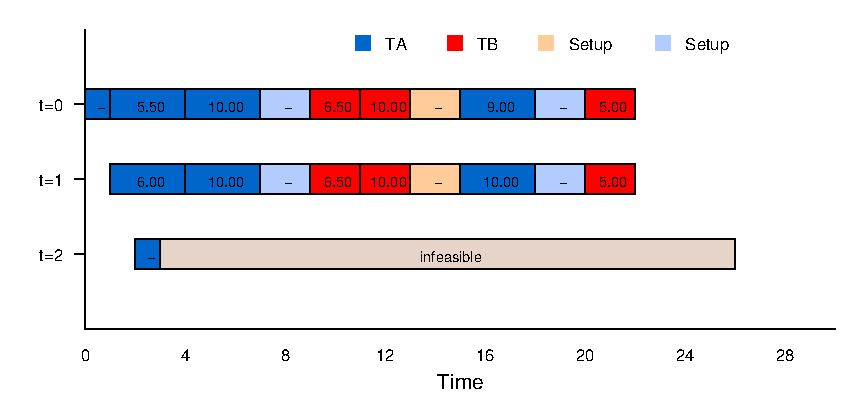
\includegraphics{scheduling/gantt_NT.pdf}
\caption{Rescheduling leads to infeasibility when no backorders are allowed}
\label{fig:scheduling:gantt_NT}
\end{center}
\end{figure}

\begin{alignat}{2}
\label{eq:scheduling:Periodic}
\mathbb{P}_P:& \min_{\bu,x(0)}{\sum_{t=0}^{N_P-1}
  \ell_E(x(t),u(t),d^{\text{nom}}(t))} &\nonumber \\ 
&\text{s.t.~} x(t+1) = Ax(t) + Bu(t)+B_dd^{\text{nom}}(t), &\qquad t = \set{0,1,\ldots,N-1}\nonumber\\
&\underline{b} \leq E_xx(t) + E_u u(t) \leq \bar{b},& \qquad t = \set{0,1,\ldots,N-1}  \\
& x(0) = x(N_p)& \nonumber
\end{alignat}

The Gantt chart for the periodic solution is shown in Figure
\ref{fig:scheduling:gantt_Periodic}. 

\begin{figure}
\begin{center}
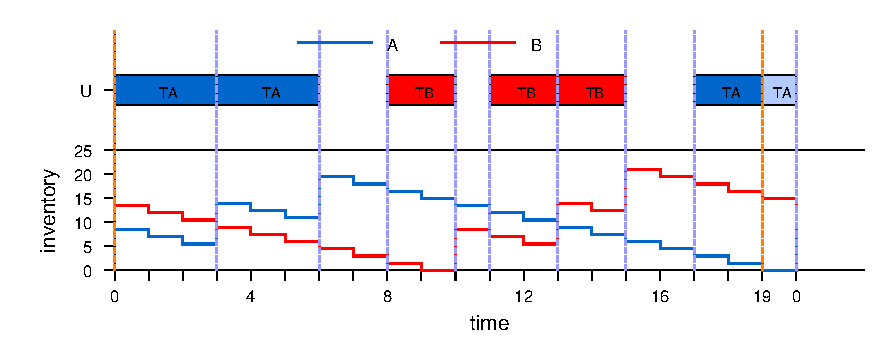
\includegraphics{scheduling/gantt_Periodic.pdf}
\caption{Periodic solution  for the example in the absence of disturbances}
\label{fig:scheduling:gantt_Periodic}
\end{center}
\end{figure}

We now illustrate the use of terminal constraints on the states of the
model which enable us to retain feasibility of the scheduling problem
as we roll the horizon forward. To do so, we use the cyclic schedule
found by optimization problem \eqref{eq:scheduling:Periodic}. Let the
solution of the \eqref{eq:scheduling:Periodic} be given as $(x_P^0(0),
u_P^0(0), u_P^0(1), \ldots, u_P^0(N_p-1))$. For this optimal periodic
solution, we can calculate the corresponding state-evolution using the
state evolution equation. Denote the states in this optimal periodic
state evolution as
$\set{x_P^0(0),x_P^0(1),\ldots,x_P^0(N_p-1)}$. Then the optimization problem
with terminal constraints $\mathbb{P}_N^T(x)$ can be written as:
\begin{alignat}{2}
\label{eq:scheduling:T}
\mathbb{P}_N^T(x):&
\min_{\bu}{\sum_{t=0}^{N-1}\ell_E(x(t),u(t),d^{\text{nom}}(t))}&
\nonumber \\ 
&\text{s.t.~} x(t+1) = Ax(t) + Bu(t)+B_dd^{\text{nom}}(t),& t = \set{0,1,\ldots,N-1} \nonumber\\
&\underline{b} \leq E_xx(t) + E_u u(t) \leq \bar{b},& t = \set{0,1,\ldots,N-1} \\
& x(0) = x &\nonumber\\
& x(N) \in \set{x_P^0(0),x_P^0(1),\ldots,x_P^0(N_p-1)}&\nonumber
\end{alignat}

In optimization problem $\mathbb{P}_N^T$, we enforce the condition
that the terminal state be one of the states in the optimal periodic
state evolution. Therefore, the solutions to \eqref{eq:scheduling:T}
contains long-term information. This is because, we terminate at a
state from which we can implement a periodic solution to respond to
nominal demands. The Gantt chart obtained by successive
re-optimization using problem \eqref{eq:scheduling:T} is shown in
Figure \ref{fig:scheduling:gantt_Terminal}. Due to design of the
optimization problem, we remain feasible at all times. Note that the
batch of $\text{TA}$ at $t=1$ was 8 tons, because of the information
regarding future demands contained in the terminal constraint. Figure
\ref{fig:scheduling:T_24_CL} shows the closed-loop solution over 24h.

\begin{figure}
\begin{center}
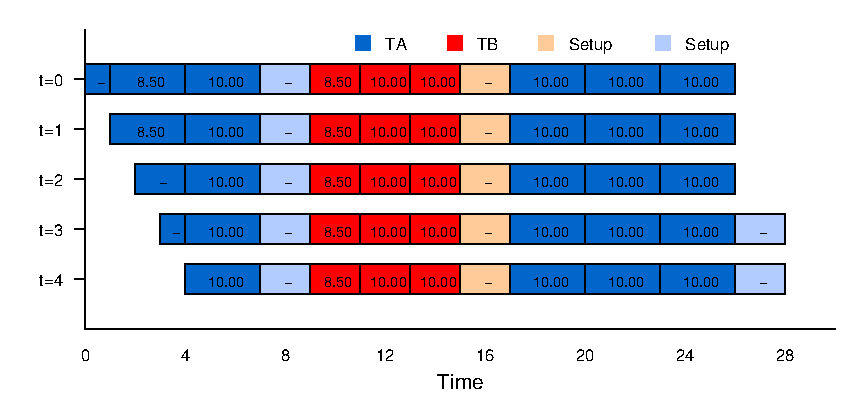
\includegraphics{scheduling/gantt_24.pdf}
\caption[Recursive feasibility with terminal constraints]{Solutions
  obtained by solving Problem \eqref{eq:scheduling:T} 
at $t=0,1,3$ and $4$. Addition of terminal constraints leads to
feasible problems. Compare the schedule at $t=0$ with
\ref{fig:scheduling:gantt_NT}. A larger batch of TA starts at $t=1$
and there are fewer changeovers, thus larger production.}
\label{fig:scheduling:gantt_Terminal}
\end{center}

\end{figure}
\begin{figure}

\begin{center}
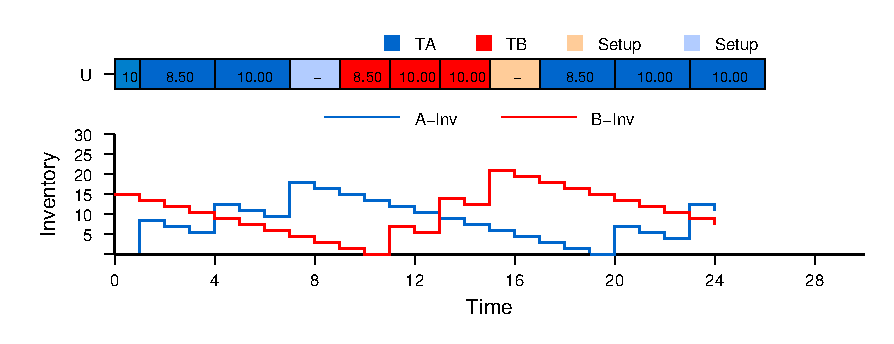
\includegraphics{scheduling/T_24_CL.pdf}
\caption{Closed-loop solution solving \eqref{eq:scheduling:T} with
  $N=24h$}
\label{fig:scheduling:T_24_CL}
\end{center}
\end{figure}

We can use terminal constraints to reduce the computational burden in
scheduling because, as shown in Figure \ref{fig:scheduling:gantt_12},
we can guarantee recursive feasibility using shorter prediction
horizons also. In Figure
\ref{fig:scheduling:gantt_12}, Problem \eqref{eq:scheduling:T} was
solved with $N=12$ and Figure \ref{fig:scheduling:T_12_CL} shows the closed-loop
solution over a horizon of 24h using a prediction horizon of $12h$.

 
\begin{figure}
\begin{center}
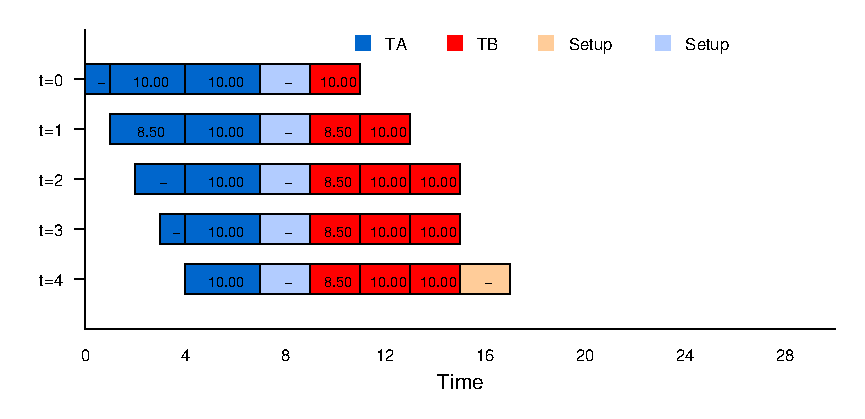
\includegraphics{scheduling/gantt_12.pdf}
\caption[Recursive feasibility with terminal constraints for
$N=12h$]{Solutions obtained by solving Problem \eqref{eq:scheduling:T} 
at $t=0,1,3$ and $4$. Recursive feasibility is maintained with proper
choice of terminal constraints}
\label{fig:scheduling:gantt_12}
\end{center}
\end{figure}
\begin{figure}

\begin{center}
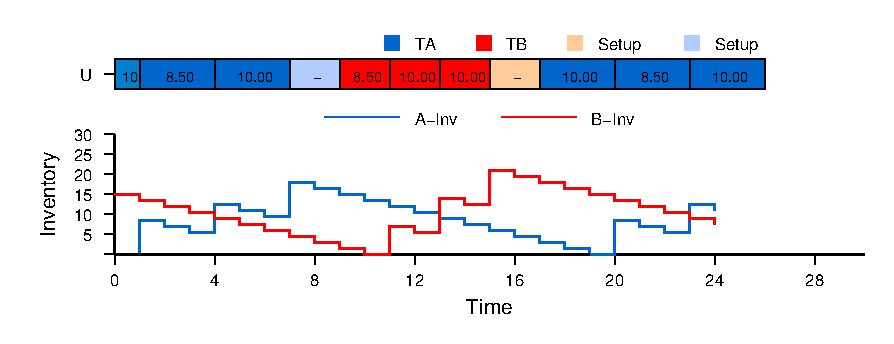
\includegraphics{scheduling/T_12_CL.pdf}
\caption{Closed-loop solution solving \eqref{eq:scheduling:T} with
  $N=12h$}
\label{fig:scheduling:T_12_CL}
\end{center}
\end{figure}

\subsection{Rescheduling}
In this section, we consider the same model as in Section
\ref{sec:scheduling:example:nominal}, but with backlogs. That is, we
introduce shipments $V_{k,t}$ and backlog $U_{k,t}$ with the new state
equations defined by \eqref{eq:scheduling:xbacklog} and
\eqref{eq:scheduling:backlog}. We enforce an economic penalty on
accumulating backlogs. 

The following disturbances are observed: (i) Production delay of 1h
at $t=6$, (ii) breakdown for 3h  from $t=10$ to $t=13$, (iii)
unloading error at $t=14$ (production of  B is 8ton instead of 10ton)
and, (iv) demand spike at $t=16$, with $\hat{\xi}_i = 0.5$, that is
the demand for both products were 2tons instead of the nominal demand
of 1.5 ton. Figures \ref{fig:scheduling:gantt_NT_disturbance} and
\ref{fig:scheduling:CL_NT_disturbance} shows the closed-loop
performance for an optimizer optimizing \eqref{eq:scheduling:NT}. We
can observe the rescheduling that occurs naturally using the rolling
horizon framework in Figure
\ref{fig:scheduling:gantt_NT_disturbance}. For example, the batch
sizes change between $t=6$ and $t=7$ and $t=14$ and $t=15$ after the
realization of disturbances. Finally, Figure
\ref{fig:scheduling:CL_T_disturbance} shows the closed-loop response
for the same disturbances, but when the optimizer was solving
\eqref{eq:scheduling:T}; that is, when we were enforcing terminal
cyclic constraints. We observe  inherent robustness of the
terminal constraint formulation as the backlogs accumulated are
lesser than the formulation without terminal constraints. 
\begin{figure}
\begin{center}
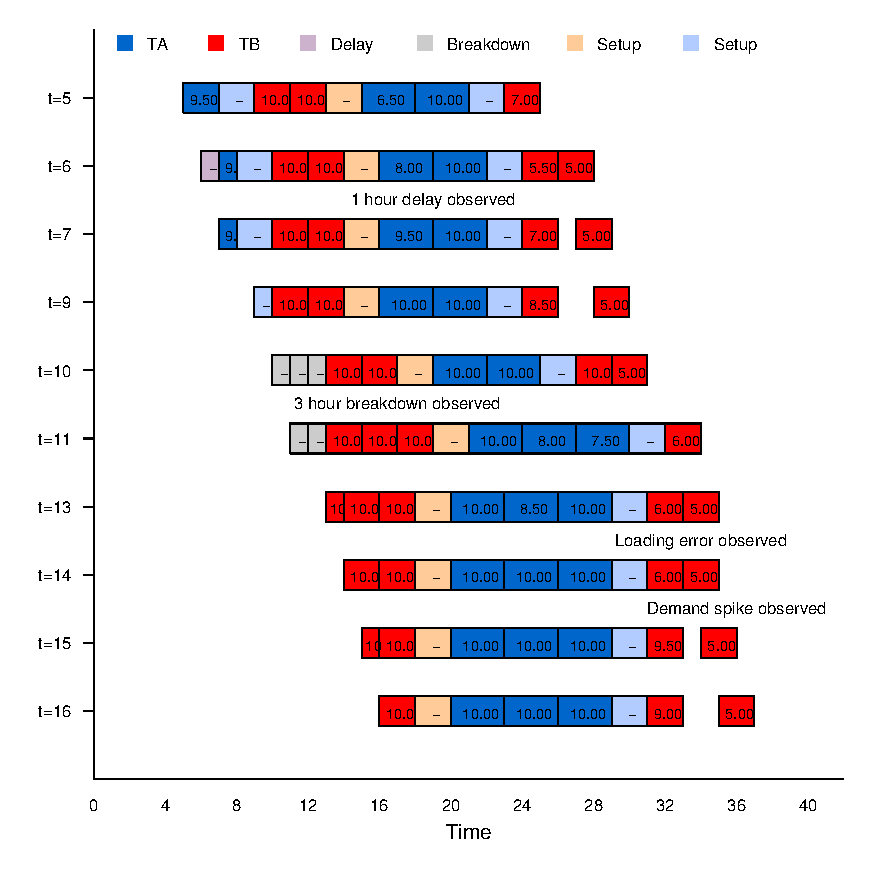
\includegraphics{scheduling/gantt_NT_disturbance.pdf}
\caption{Rescheduling in the presence of disturbances}
\label{fig:scheduling:gantt_NT_disturbance}
\end{center}
\end{figure}

\begin{figure}
\begin{center}
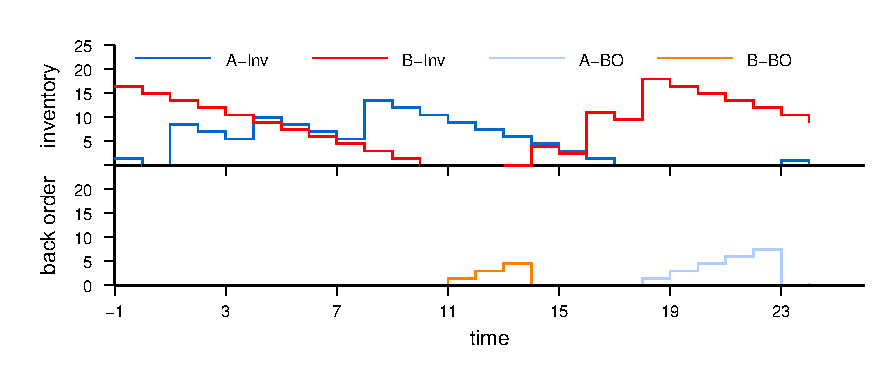
\includegraphics{scheduling/CL_NT_disturbance.pdf}
\caption[Closed-loop with disturbances]{Inventory (Inv) and Backorder(BO) profiles in the closed-loop
  in the presence of disturbances.}
\label{fig:scheduling:CL_NT_disturbance}
\end{center}
\end{figure}


\begin{figure}
\begin{center}
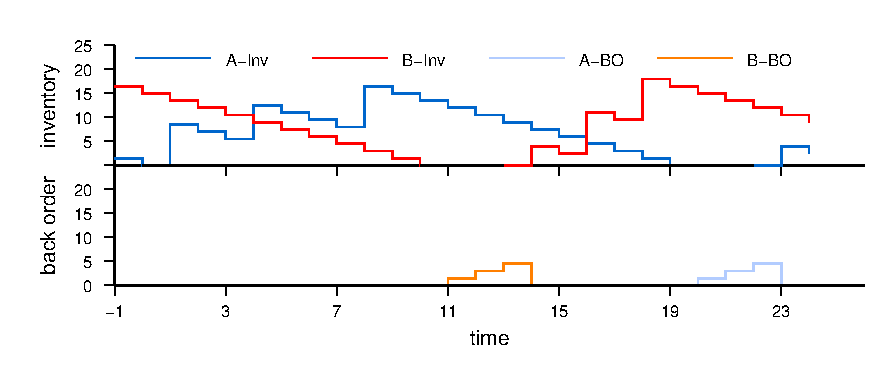
\includegraphics{scheduling/CL_T_disturbance.pdf}
\caption[Closed-loop for terminal constraint formulation with disturbances]{Inventory (Inv) and Backorder(BO) profiles in the closed-loop
  in the presence of disturbances. Compare with
  \ref{fig:scheduling:CL_NT_disturbance} to notice the inherent
  robustness of the terminal constraint formulation}
\label{fig:scheduling:CL_T_disturbance}
\end{center}
\end{figure}




\section{Discussion}
\subsection{Generality of the scheduling model\footnote{This text appears in Section 3.5.1 of \citet{subramanian:maravelias:rawlings:2012}}}

Most current approaches to reactive scheduling are based on scheduling
models that do not include disturbances explicitly. Thus, when an event
triggers rescheduling, an empirical procedure is followed to modify the
scheduling model so it (i) represents the new state of the system, and
(ii) accounts for the future impact of the disturbance. One advantage
of the state space model is that the same model can be directly used
for rescheduling. All events that can trigger rescheduling are modeled
via disturbance variables. Thus, for a resolve it is sufficient to fix
the appropriate disturbance variables, which can be readily calculated
from the observation at the current time. No empirical model
modifications are necessary.

\subsection{Stochastic vs. deterministic approaches\footnote{This text appears in Section 3.5.2 of \citet{subramanian:maravelias:rawlings:2012}}}

In this paper, we treat scheduling as an on-line problem; we optimize
to determine a single schedule based on current data and forecasts,
and as new information becomes available we re-optimize to determine,
again, a single solution. In each re-optimization, we solve a
deterministic problem- we do not account for the fact that some data
are subject to uncertainty that can be modeled. An alternative
approach is to model the uncertainty in the events that can trigger
rescheduling, and then generate a solution that takes into account
this information \citep{li:ierapetritou:2008b,sahinidis:2004}. The
obvious advantage of this so-called {\em{optimization under
    uncertainty}} approach is that, if the model is solved
effectively, then it can lead to better solutions. The disadvantage is
that most optimization under uncertainty methods are computationally
expensive, and thus cannot be used to address practical
problems. Robust optimization methods have been proposed to address
this shortcoming
\citep{ben-tal:nemirovski:2002,verderame:floudas:2009}; they rely on
solutions that is almost as hard as the deterministic problem, but
leads to solutions that are conservative. The advantage of the
control-inspired approach that we follow is that the deterministic
optimization problem can be solved more effectively, which has three
implications. First, it can lead to optimal (or near optimal)
solutions that are better (even when evaluated under uncertainty) than
the solution that can be obtained within the same time by a stochastic
programming approach. Second, it allows us to reschedule more
frequently, thus reacting faster to disturbances and thereby resulting
in better closed-loop solution. Third, it allows us to consider longer
scheduling horizons, which is critical and can often be more
important that accounting for uncertainty.

\subsection{Types of disturbances and uncertainties\footnote{This text appears in Section 3.5.3 of
  \citet{subramanian:maravelias:rawlings:2012}. Equation
  \eqref{eq:scheduling:discussion} has been modified to remain
  consistent with the notation used in this chapter}}

Interestingly, the types of disturbances we have discussed
correspond, when treated as stochastic parameters, to different types
of uncertainty. Shipment disturbances can be viewed as right-hand side
(RHS) uncertainty. Production and consumption disturbances can be
viewed as left-hand side (LHS) uncertainty, since they can be treated
as uncertainties in the $\beta_{ik} = \rho_{ik}\beta_i$ terms:

\begin{equation}
\label{eq:scheduling:discussion}
S_{k,t+1} = S_{k,t}+ \sum_{i \in
  \mathbb{I}^+}(\beta_{i}\bar{W}_{i,t}^{n}+\beta_{i,k,t}^P)\rho_{ik}
+\sum_{i \in
  \mathbb{I}^-}(\beta_{i}{W}_{i,t}+\beta_{i,k,t}^C)\rho_{ik} +
\zeta_{k,t} \qquad \forall k,t
\end{equation}

These are two types of uncertainty that have received the most
attention in stochastic optimization approaches to scheduling.

Task delays can also be treated as LHS uncertainty if the duration of
a task appears only as a LHS coefficient (in the case of fixed
processing times) or as a variable defined in terms of stochastic
parameters (in the case of variable processing
times). Precedence-based models or time-grid based models with
continuous modeling of time may result in stochastic optimization
problems which lead to LHS uncertainty. However, in discrete-time
formulations, the number of terms included in the summation in the LHS
of the assignment constraint depends on the duration of a task. Thus,
in this case, the treatment of task delays through the modeling of
processing times as stochastic parameters leads to a
{\emph{structural}} type of uncertainty.

Finally, unit breakdowns lead to structural uncertainty since the
constraints used to model resource constraints should be removed or
modified. Stochastic optimization approaches cannot be used to
effectively address this type of structural uncertainty because, in
addition to requiring on-the-fly reformulations of the scheduling
model, task delays and unit breakdowns lead to problems with either
{\emph{purely endogenous}} uncertainty or {\emph{exogenous uncertainty
    with endogenous observation}} \citep{colvin:maravelias:2008,colvin:maravelias:2010,goel:grossmann:2006}. For example, the
  probability and the timing of a unit breakdown depends on the
  utilization of the unit, which is determined by the decision
  maker. The proposed approach does not suffer from this limitation. 

\subsubsection{Reverse transformation and reoptimization\footnote{This text appears in Section 3.5.2 of \citet{subramanian:maravelias:rawlings:2012}}}

Since scheduling MIP models are computationally expensive, a potential
disadvantage of the proposed state space modeling framework is that it
leads to MIP models of larger size. For example. compared to its
counterpart model, $\mathbf{M}^{\text{SCH}}$, model
$\mathbf{M}^{\text{MPC}}$, has additional lifted variables (lifted
inputs $\bar{W}_{i,t}^{n}$) and
equations \eqref{eq:scheduling:liftedW}. However, model $\mathbf{M}^{\text{MPC}}$
is not significantly slower than $\mathbf{M}^{\text{SCH}}$. First we
note that the addition of disturbance variables in Equations
\eqref{eq:scheduling:finalSS} and
\eqref{eq:scheduling:breakdown_constraint} leads to changes in RHS
constant vector $b$, if the optimization model is written as
$\max_{}{\set{c'x: Ax \leq b. x \in \mathbf{X}}}$. In other words,
they do not increase the complexity of the model. Second, the lifting
equations can be used to project out variables after the state of the
system is updated using $\mathbf{M}^{\text{MPC}}$ and before
reoptimization is performed. Commercial MIP solvers perform this type
of preprocessing (variable elimination and constraint removal) automatically
\citep{atamturk:savelsbergh:2005}. Third, specific preprocessing
methods can be easily developed to transform the {\emph{current}}
$\mathbf{M}^{\text{MPC}}$ model (i.e. the model after the injection of
disturbances at $t$) back to a model in the form
$\mathbf{M}^{\text{SCH}}$. Perprocessing based on
$\mathbf{M}^{\text{MPC}}$ can also be used to automatically detect
what constraints should be removed or modified. For example. in the
case of a breakdown of unit $j=U$ from $t_1$ to $t_2$, the constraint
\eqref{eq:scheduling:breakdown_constraint} becomes:
\[ \sum_{i\in \mathbf{I}_j}W_{i,t} + \sum_{i \in
  \mathbf{I}_j}\sum_{n=1}^{\tau_i-1} \bar{W}_{i,t}^{n} \leq 0 \qquad
\forall t \in \set{t_1,\ldots,t_2-1}
\] 
which mathematically implies that all binary variables appearing in
the LHS should be fixed to zero and Equation
\eqref{eq:scheduling:breakdown_constraint} be removed from the model
for $j=U$ and $t\in \set{t_1,\ldots,t_2-1}$. Not surprisingly, this is
what one would do using logical arguments: if there is a breakdown in
an unit, then no tasks can be started on this unit (i.e., all binaries
are set to zero), and thus the corresponding assignment constraint can
be removed. Model $\mathbf{M}^{\text{MPC}}$ allows us to
systematically perform this type of reasoning. We note that our
preliminary computational experience confirms that
$\mathbf{M}^{\text{MPC}}$ is computationally comparable with model
$\mathbf{M}^{\text{SCH}}$. 


Finally, lifting the inputs offers
insights into generation of the models for rescheduling. As we saw,
the current state of the system includes past inputs from
$t-\max_i{\tau_i}$ to $t$. Hence, when reformulating original model
$M^{\text{SCH}}$, we have to fix the decisions made in the last
$\max_i{\tau_i}$ periods. This approach has been proposed in the past
\citep{sundaramoorthy:maravelias:2010}. The use of state space models
and input lifting formalizes this approach and makes it easy to write
rescheudling model for any disturbance. 

\subsection{MPC tools\footnote{This text appears in Section 6.1 of \citet{subramanian:maravelias:rawlings:2012}}}

The development of a state space model is a first step towards the use
of MPC theory and methods to address scheduling problems. It offers a
representation of scheduling problems with which the process control
community is familiar. Since scheduling is a dynamic problem and can
be viewed as a {\emph{production}} control problem, our hope is that
the proposed framework will enable MPC technology for scheduling
problems. 

Another outcome is that if facilitates the application of methods that
have been developed for hybrid dynamic systems consisting of both time
and event driven dynamics \citep{bemporad:morari:1999,
  heemels:schutter:bemporad:2001}. Control of such systems has been the
focus of many researchers in the past decade (see \citep{camacho:ramirez:limon:pena:alamo:2010} for a
review of MPC techniques for hybrid systems). At the same time,
studying this new class of problems can lead to the development of new
tools for hybrid system.

The state space model can also help to bridge the gap between
scheduling and control since it allows the formulation of the
integrated scheduling-control problem using a state space
model. Furthermore, the unified problem can be viewed as an economic
MPC problem in which the process economics (primarily determined by
the scheduling decisions) are directly optimized by the controller \citep{diehl:amrit:rawlings:2011}.

More importantly. it offers a natural framework for the development
of new scheduling algorithms based on MPC. As mentioned in Section
\ref{sec:scheduling:introduction}, scheduling is still thought of as
an open-loop problem, even though it is used in an iterative
manner. As a results, concepts such as stability,
recursive-feasibility, and closed-loop performance have received no
attention. In Section \ref{sec:scheduling:example}, we showed how
terminal constraints can be used to guarantee recursive feasibility.





%end chapter
